\documentclass{article}
\usepackage{hyperref}
\usepackage{amsmath, amssymb, graphicx}
\usepackage[a4paper, margin=0.7in]{geometry} % Adjust margins

\title{Implementation of Adaptive Step-Size for Convex Optimization}
\author{
    Ali Ghasemzadeh - 401106339 \\
    Armin Khosravi - 401105872 \\
    Donya Jafari - 401101524
}

\date{\today}

\begin{document}
\maketitle

\section{Introduction}

This report presents the implementation of the adaptive step-size optimization algorithm proposed in 
\href{https://www.dcsc.tudelft.nl/~mohajerin/Publications/journal/2024/adap_stepsize.pdf}
{\textit{Adaptive Accelerated Composite Minimization}}. The algorithm considers different cases based on acceleration and composite structures. The convergence details and theoretical analysis are provided in the original paper.

\section{Formulas}

The key formulas used in the adaptive step-size method are as follows:

\[
x_{k+1} = x_k + \lambda_k d_k,
\]

where

\[
\varphi_k(\lambda) := f(x_k + \lambda d_k).
\]

For a general optimization problem:

\[
F(x) = \min_{x \in X} \left( f(x) \right) + h(x),
\]

the adaptive step size is determined by:

\[
\lambda_k := \arg\max_{\lambda} \lambda \quad \text{such that the inequalities in the table below hold}.
\]

The proximal operator is defined as:

\[
\text{prox}_h(x) = \arg\min_u \left( h(u) + \frac{1}{2} \|u - x\|^2 \right),
\]

and the gradient mapping is:

\[
G_{\lambda h}^f(x) := \frac{1}{\lambda} \left( x - \text{prox}_{\lambda h}(x - \lambda \nabla f(x)) \right).
\]

Below is a table summarizing the step size rules and convergence rates for different settings:

\[
\begin{array}{|c|c|c|c|}
\hline
\textbf{Algorithm} & \textbf{Problem} & \textbf{Stepsize Rule} \\
\hline
\text{Non-accelerated} & \text{Composite} & \varphi(2\lambda) \leq \varphi(\lambda) - \lambda (G_{\lambda h}^f(x), \nabla f(x)) + \frac{\lambda}{2} \|G_{\lambda h}^f(x)\|^2  \\
\text{Non-accelerated} & \text{Smooth} & \varphi(2\lambda) \leq \varphi(\lambda) + \frac{\lambda}{2} \varphi'(0)  \\
\text{Accelerated} & \text{Composite} & \varphi(2\lambda) \leq \varphi(\lambda) - \lambda (G_{\lambda h}^f(x), \nabla f(x)) + \frac{\lambda}{2} \|G_{\lambda h}^f(x)\|^2  \\
\text{Accelerated} & \text{Smooth} & \varphi(2\lambda) \leq \varphi(\lambda) + \frac{\lambda}{2} \varphi'(0) \\
\hline
\end{array}
\]

\section{Problem List and Implementation}
The following problems were implemented and tested:

\begin{enumerate}
    \item Logistic Regression
    \item Quadratic programming
    \item Log-Sum-Exp
    \item Approximate Semidefinite Programming for the Max-Cut problem
    \item $\ell$1-Regularized least square
    \item $\ell$1-Constrained least square
    \item $\ell$1-Regularized logistic regression
    \item $\ell$1-Regularized least square (acc)
    \item $\ell$1-Regularized logistic regression (acc)


\end{enumerate}

For each problem, we provide two plots: one showing the function value convergence and another depicting step-size evolution.

\subsection{Non-Accelerated Cases}
The first set of experiments evaluates the non-accelerated versions of the algorithm across all seven problems.

\begin{figure}[htbp]
    \centering
    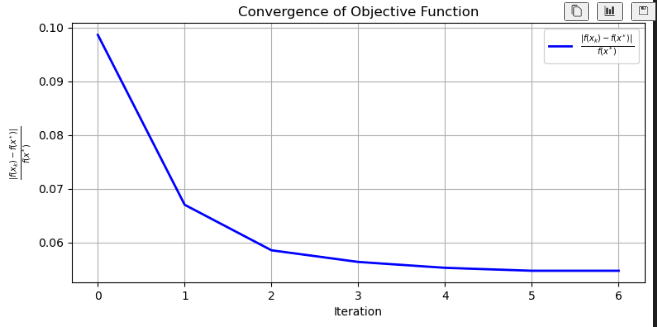
\includegraphics[width=0.4\textwidth]{11.png}
    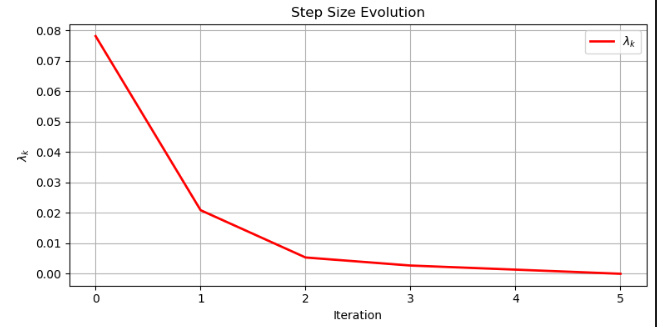
\includegraphics[width=0.4\textwidth]{12.png}
    \caption{Results for Logistic Regression (Non-Accelerated)}
\end{figure}

\begin{figure}[htbp]
    \centering
    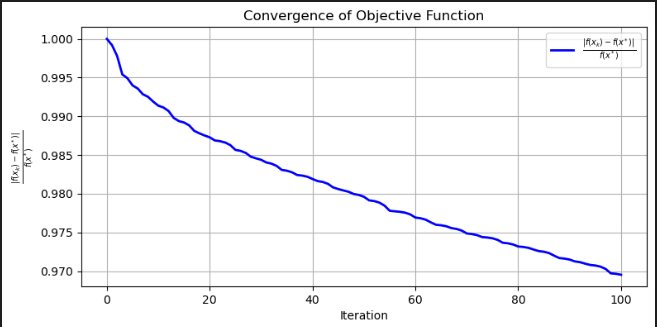
\includegraphics[width=0.4\textwidth]{21.png}
    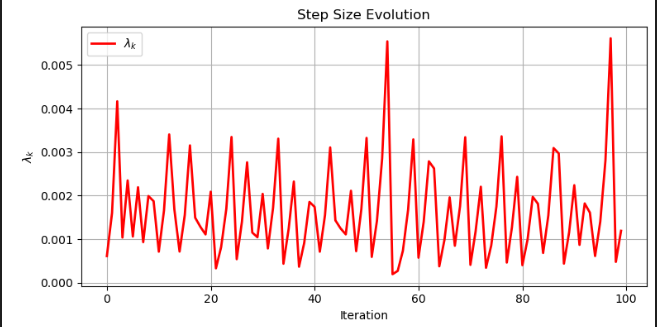
\includegraphics[width=0.4\textwidth]{22.png}
    \caption{Results for Quadratic Programming (Non-Accelerated)}
\end{figure}

\begin{figure}[htbp]
    \centering
    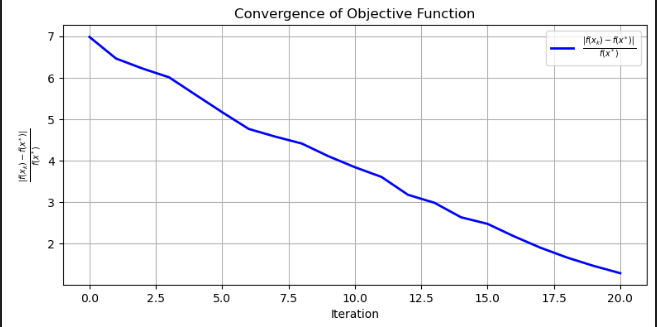
\includegraphics[width=0.4\textwidth]{31.png}
    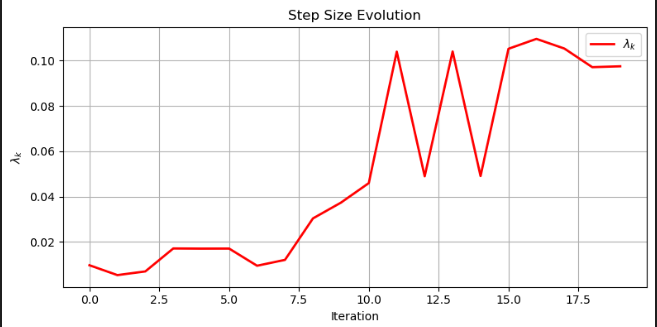
\includegraphics[width=0.4\textwidth]{32.png}
    \caption{Results for Log-Sum-Exp (Non-Accelerated)}
\end{figure}

\begin{figure}[htbp]
    \centering
    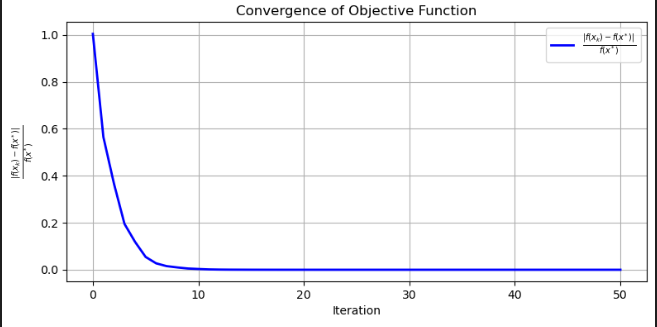
\includegraphics[width=0.4\textwidth]{41.png}
    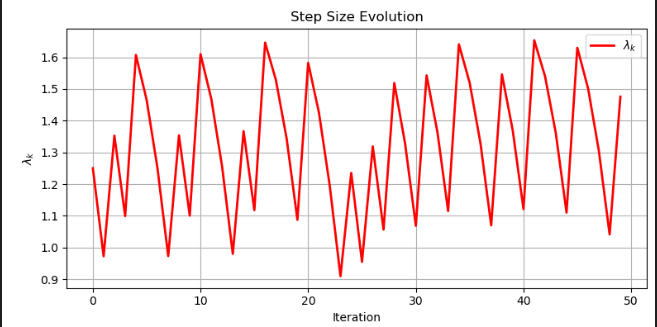
\includegraphics[width=0.4\textwidth]{42.png}
    \caption{Results for  Max-Cut problem (Non-Accelerated)}
\end{figure}

\begin{figure}[htbp]
    \centering
    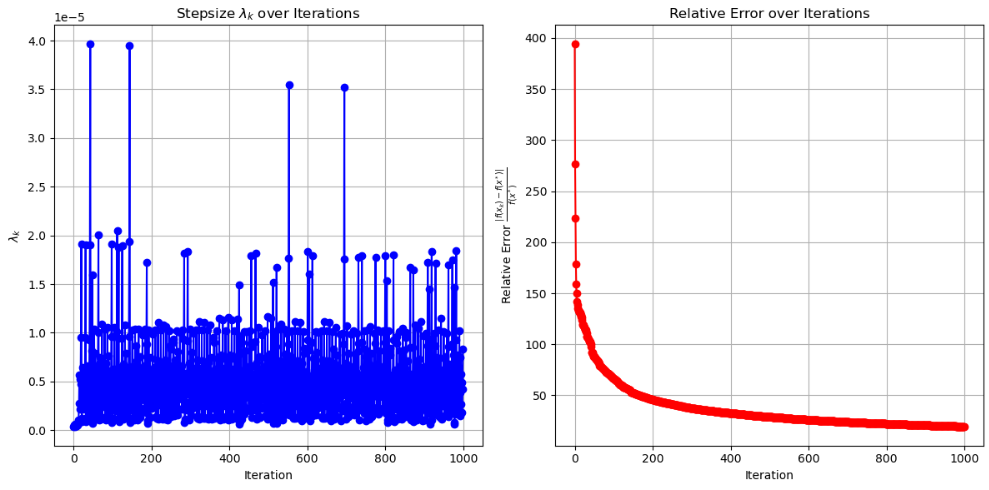
\includegraphics[width=0.6\textwidth]{5.png}
    \caption{Results for $\ell$1-Regularized least square (Non-Accelerated)}
\end{figure}


\begin{figure}[htbp]
    \centering
    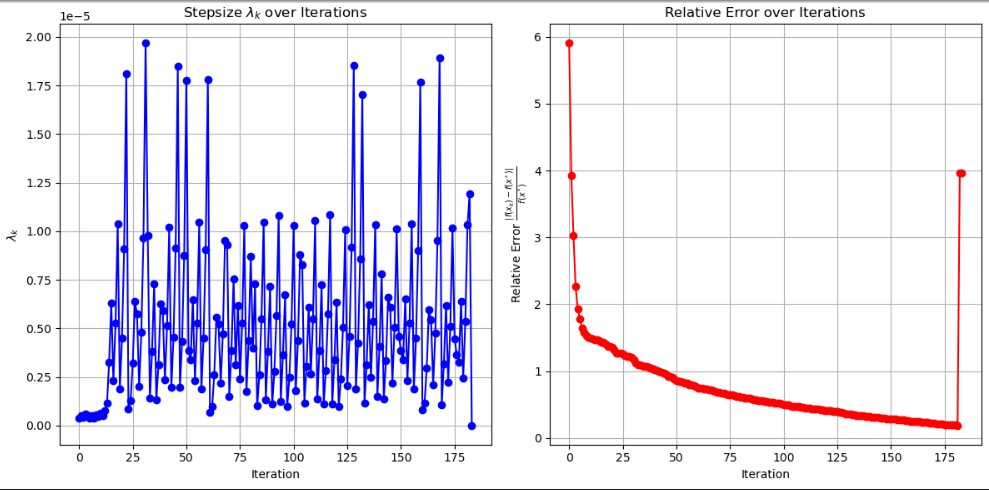
\includegraphics[width=0.6\textwidth]{6.png}
    \caption{Results for $\ell$1-Constrained least square (Non-Accelerated)}
\end{figure}


\begin{figure}[htbp]
    \centering
    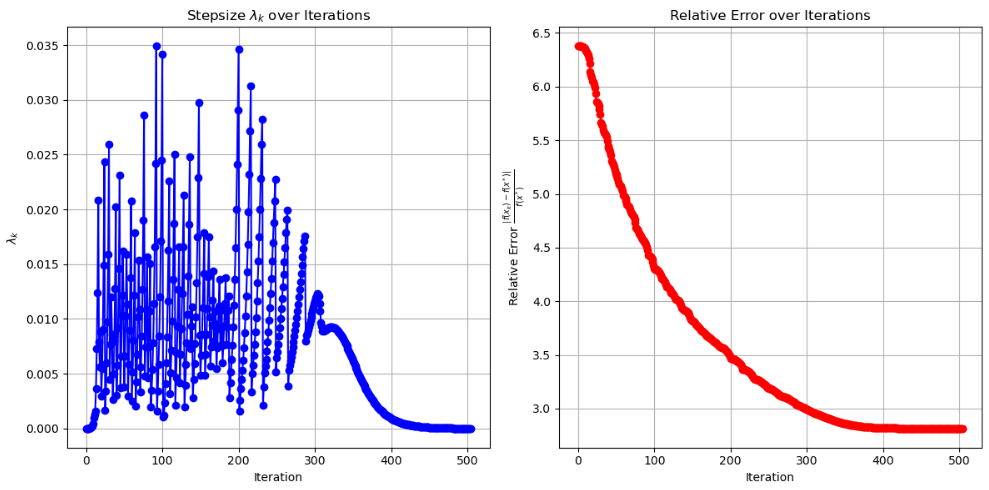
\includegraphics[width=0.6\textwidth]{7.png}
    \caption{Results for $\ell$1-Regularized logistic regression (Non-Accelerated)}
\end{figure}


\clearpage 


% Add additional figures for each problem in the list as needed

\subsection{Accelerated Cases}
Acceleration was applied only to two of the convex problems. The results are presented below.

\begin{figure}[htbp]
    \centering
    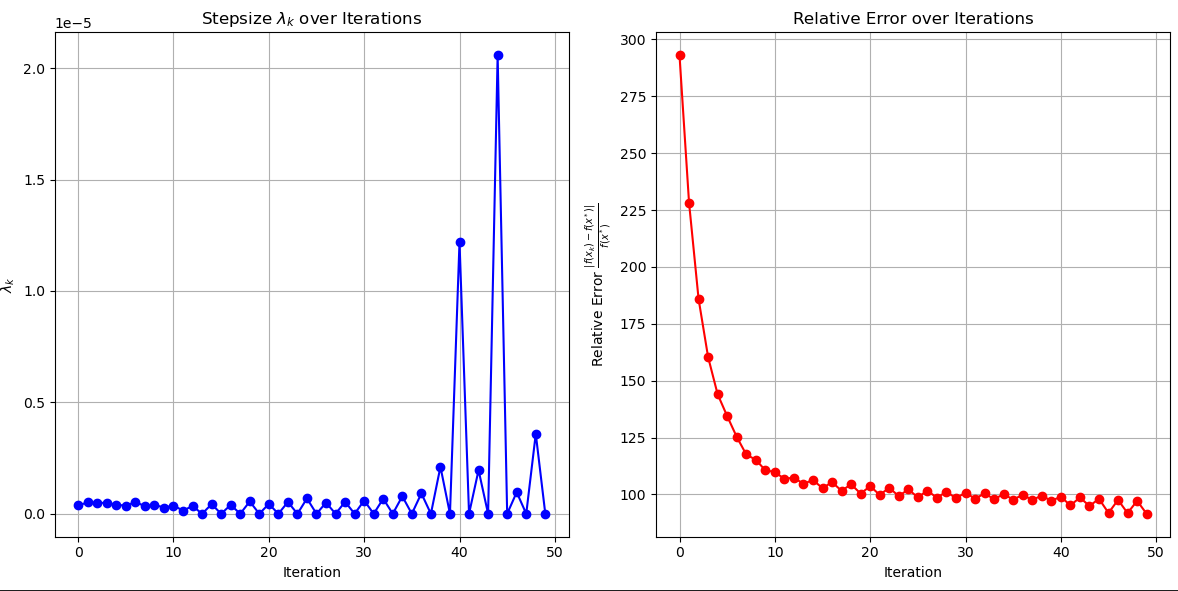
\includegraphics[width=0.6\textwidth]{8.png}
    \caption{Results for $\ell$1-Regularized Least Square (Accelerated)}
\end{figure}

\begin{figure}[htbp]
    \centering
    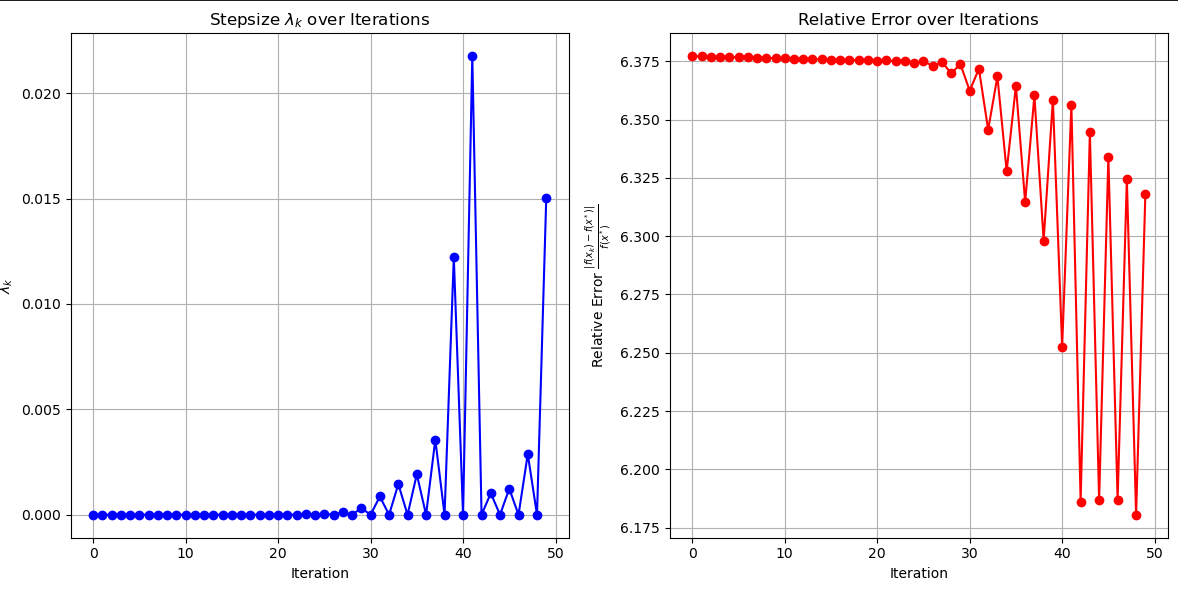
\includegraphics[width=0.6\textwidth]{9.png}
    \caption{Results for $\ell$1-Regularized logistic regression (Accelerated)}
\end{figure}

\section{Initialization and Backtracking}
The initial value of the step size, $\lambda_0$, is determined by:

\[
\lambda_0 = {2} \left( \frac{f(x_{k - 1}) - f(x_k)}{\|\nabla f(x_k)\|^2} \right).
\]

Backtracking is then used to find the largest step size $\lambda$ such that the condition holds. For the smooth case, the direction is given by the gradient, and for the composite case, the direction is $-G$.

For accelerated composite cases, we used:

\begin{figure}[htbp]
    \centering
    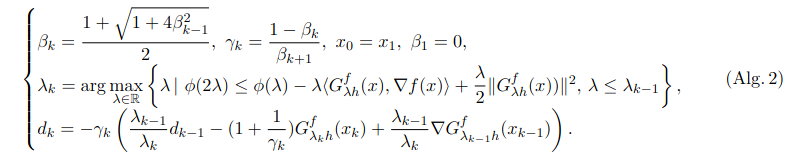
\includegraphics[width=1\textwidth]{image.png}
    \caption{Accelerated update rule (there is a typo in the gradient of G. we only need G here)}
\end{figure}

\section{Results and Discussion}
The results indicate that the adaptive step-size method effectively optimizes the convex problems. The impact of acceleration is observed in faster convergence for the selected problem.

\begin{thebibliography}{9}
    \bibitem{mohajerin2024} M. Mohajerin Esfahani, et al., "Adaptive Step-Size Methods for Convex Optimization," 2024.
\end{thebibliography}

\end{document}
